\section{Introduction}
%Software tends to accrue features and complexity over time \cite{Adar2014, Li2011, McGrenere2002, MM-gi2000}. This bloat creates a steep learning curve in four ways: First, novice users often have a different vocabulary than the application \cite{Adar2014}, making it difficult to locate desired features. Second, while online tutorials abound, they can be hard to follow and users must interpret and adapt them to suit their situation and goals \cite{Kelleher2005}. Third, software often provides several strategies for accomplishing similar tasks. Some are faster, easier, or more effective than others, and it can be difficult to identify which these are. Finally, users are typically only aware of a small percentage of software features \cite{MM-gi2000}; there may be potential results they could achieve but do not think to try.

Accomplishing one's goal with software generally requires composing multiple operations into a sequence. The burden is on the user to know which operations to combine and how to execute them. This work aims to reduce the execution gap between users' high-level task goals and the low-level steps needed to achieve them, by suggesting action macros. These aggregated action suggestions move the user's focus from individual \textit{operations} to human-understandable, goal-driven \textit{activities} \cite{Li2008, Gay2004}.

\begin{figure}[b!]
\centering
  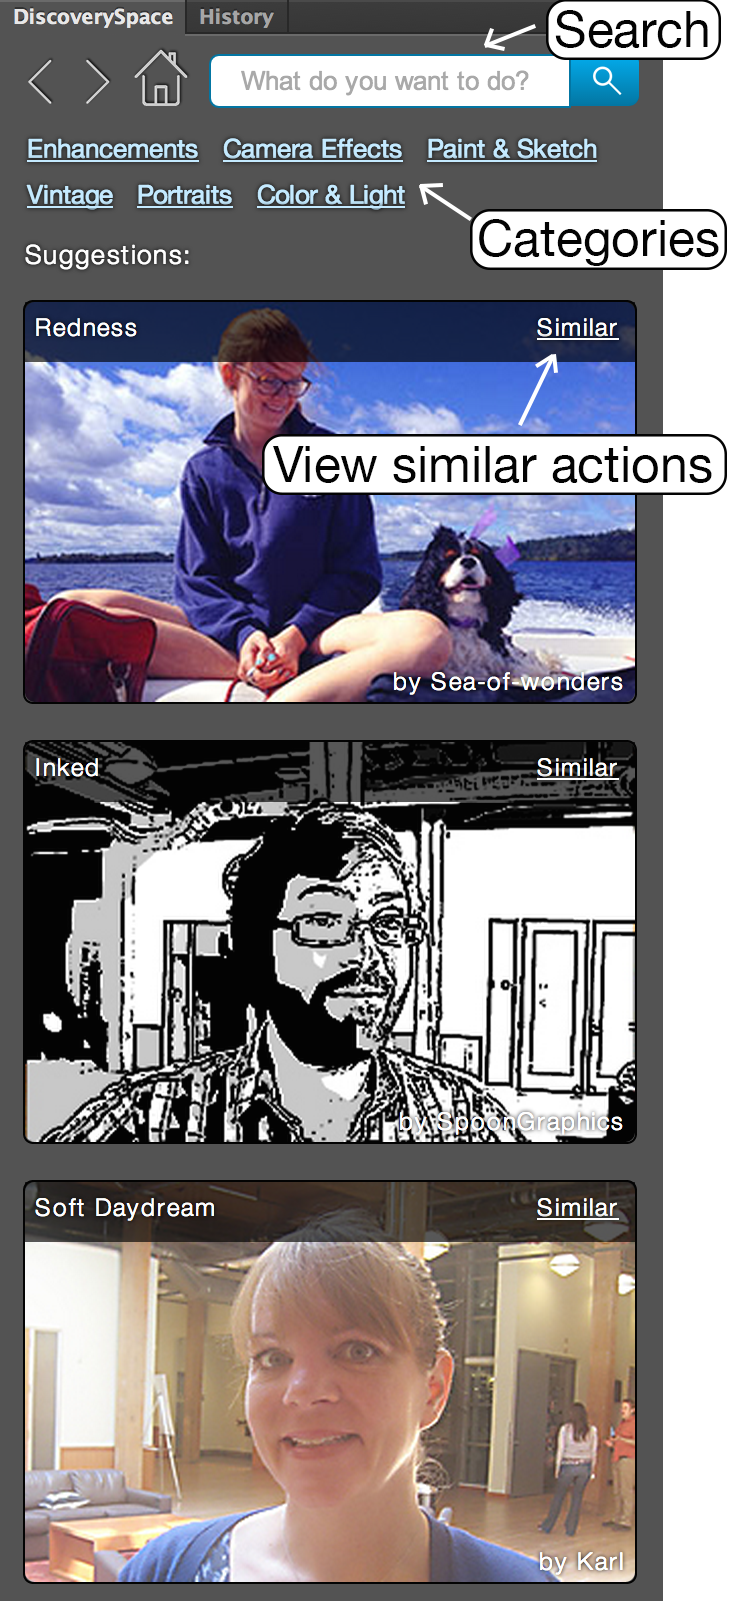
\includegraphics[width=0.35\textwidth]{discoveryspace/figures/discoveryspace_with_labels.png}
  \caption{DiscoverySpace as a panel in Photoshop. Users can apply a suggested action by clicking on its image.}~\label{fig:discoveryspace_interface}
\end{figure}

We investigate the efficacy of action suggestions through Discovery\-Space (\autoref{fig:discoveryspace_interface}), a recommendation interface for action macros recorded by the user community. Action macros encapsulate a sequence of operations that is executed as a batch, and are widely shared online\footnote{A Google search for ``free photoshop actions'' brings up over 39 million results, such as \href{https://www.creativebloq.com/photoshop/photoshop-actions-912784}{\nolinkurl{creativebloq.com/photoshop/photoshop-actions-912784}} and \href{https://fixthephoto.com/free-photoshop-actions}{\nolinkurl{fixthephoto.com/free-photoshop-actions}}.}. The Discovery\-Space prototype is a Photoshop panel comprising action macros that can be applied in one click for quick and easy exploration. We hypothesize that action suggestions help users get started in complex applications by enabling them to easily explore creative possibilities and achieve quick results.

This chapter contributes a prototype action suggestion system, Discovery\-Space, and the results of a preliminary experiment to examine its efficacy. This between-subjects study found that action suggestions may help prevent novices from losing confidence in their abilities, and help users to accomplish tasks and discover new features. This chapter also proposes design guidelines for a suggestion interface based on these observations and results.
